\leadauthor{Yangyang Li}

\title{PxBLAT: An Efficient and Ergonomics Python Binding Library for BLAT}
\shorttitle{Ergonomic Genomic Analysis with \gls{pxblat} }

\author[1]{Yangyang Li\orcidlink{0000-0001-8224-1067}}
% \author[2]{Second Doctor \orcidlink {000-0002-0000-0000}}
\author[1,\Letter]{Rendong Yang \orcidlink {000-0003-0000-0000}}
\affil[1]{Department of Urology, Northwestern University Feinberg School of Medicine, Chicago, IL 60611}
% \affil[2]{B Institute, Chalk Road, Blackboardville, USA}
\date{}

\maketitle

\begin{abstract}
	\gls{pxblat} provides an ergonomic and efficient Python binding library for \gls{blat}, designed to enhance the user experience and performance of genomic analysis tasks.
	By providing a pythonic interface to \gls{blat}, \gls{pxblat} simplifies the usage of \gls{blat}, allowing incorporating its functionality directly into their Python-based bioinformatics workflows.
	Furthermore, A new parallelization and non-blocking model enables improved efficiency and intuitive user interface, thereby reducing the complexity of genomic data analysis tasks.
\end{abstract}


\begin{keywords}
	Software Libraries |  Sequence Analysis | BLAT
\end{keywords}

\begin{corrauthor}
	rendong.yang\at northwestern.edu
\end{corrauthor}

\section*{Introduction}\label{sec:introduction}



% % NOTE: Pyblat <05-08-23, Yangyang Li>

% Realig nment is the process that mapping certain sequence to reference since the alignment result getting from aligner may be not accurate.
% We want to get precise alignment result  by realignment.
% Blat, which is realignment tool provided by UCSC,  aims for mapping sequences to reference.
% It also provides another version of blat that provide two separate tools.
% The two tools can start a server based on certain reference first and then query sequence toward sever as long as the server is ready.
% This method achieve huge performance improvement compared to original blat version.
% Also, Performance-aware algorithm  will need high efficient strategy to realignment.
% The server version of blat is a good choice.
% However, the UCSC only provides command line versions, which is not useful for developing  algorithm involving realignment.
% That means you need to use the blat thought system.
% Meanwhile, Getting the information from server is not  trivial as you need to communicate with log file of server.
% Hence, we need to check the log file consistently, which is mistakeful and unefficient.
% We develop a Python bindings library PyBlat based on blat and provide richer features for realignment.
% PyBlat is developed in terms of blat source code that implemented by C.
% We create Cpp version  for related functions and then use pybind11 to bind cpp code to python code.
% Besides, the library will not abort due to error from c or cpp code.
% Pyblat do not  generate any intermediate files and follow pythonic coding style.


The continual advancement of genome sequencing technologies has led to an exponential increase in available genomic data.
Tools to analyze and manipulate these data have become critically important in both research and clinical contexts.
\gls{blat} ~\citep{kent2002blat} is a standout in the bioinformatics field for its capability to perform rapid genome sequence alignments.
It offers a faster alternative to \gls{blast}~\citep{altschul1990basic}  for aligning DNA sequences to the human genome ~\citep{kent2002blat}.
Despite its widespread use and acceptance in the bioinformatics community, interfacing with BLAT can present challenges, particularly when integrating it within a broader Python-based analytical pipeline.
Since \gls{blat} is implemented by C programming language and only provides a variety of utilities with a \gls{cli}.
So far, we lack a holistic approach to enhance both the performance and the usability of BLAT.

On the other hand, Python's rise as a favored programming language in bioinformatics is well-documented, due to its ease of use, extensive libraries, and versatility~\citep{perkel2015programming}.
Various binding libraries have been developed to extend Python's reach into other computing languages, improving the flexibility and interoperability of bioinformatics tools.
For instance, Biopython~\citep{cock2009biopython}, one of the most prominent bioinformatics libraries, provides interfaces to tools like \gls{blast} ~\citep{altschul1990basic}, Clustal~\citep{higgins1988clustal}, and others.
Nonetheless, to date, no comprehensive Python binding library for BLAT has been developed.

Here we propose \gls{pxblat}, a modern Python library designed to streamline and enhance the interaction with \gls{blat}, thereby making it more efficient and ergonomic.
\gls{pxblat} serves as a bridge, bringing the high-performance capabilities of \gls{blat}  into the Python environment, which is widely regarded for its readability, simplicity, and extensive library support.
By improving the usability of \gls{blat}  and seamless integration within Python, \gls{pxblat} opens up new possibilities for efficient genomic analysis.
We provide evidence of its performance improvements, demonstrate its ergonomic advantages, and discuss its potential applications in genomic research.
The overarching aim of this work is to fill the observed gap by providing a Python binding library specifically tailored for BLAT, addressing both its efficiency and ergonomic concerns.


% TODO: mention pblat and do some comparision from usage compective <05-28-23, Yangyang Li>

\section*{Implementation}\label{sec:implementation}

% introduce features of pxblat
% 1. no intermidiate files, all in memory
% 2. no system call
% 3. no bother with log files to get status of tool
% 5. no need to worry about file format
% 6. no other dependency
% 4. higher proformance and Ergonomics (compare with current blat endpoint)

The design of \gls{pxblat} follows the pythonic principles of readability and simplicity.
It is built to be intuitive, reducing the learning curve for users familiar with Python and bioinformatics tools.
In line with this, we focused on minimizing the complexity while maximizing the usability and performance.
Hence, We employ existing C codebase and reimplement utilities of \gls{blat}(V37.1) suit  including \emph{faTwoBit}, \emph{gfServer} and \emph{gfClient} \gls{cli}  using Cpp programming language~\citep{kent2002blat}.
Then, we create \gls{pxblat} via Pybind11~\citep{pybind11}.
This approach enabled direct access to the functions of the \gls{blat} program without modifying its original source code, preserving the integrity and performance of \gls{blat} while extending its capabilities.

Furthermore, \gls{pxblat} eliminate the need for intermediate files, which allow all operations to be in memory, these tools can analyze and respond to data inputs almost instantaneously.
Input and output file now become optional, which is more flexible.
Meanwhile, \gls{pxblat} reduce the need of system calls to interact with \gls{blat}, which may prevent potential safe problem.
It provides optional non-blocking operations as well, improving the overall efficiency.
Importantly, \gls{pxblat} allow fetching status of \gls{blat} without manipulating log files, especially in concurrent environment.
That means \gls{pxblat} reduce possibility of data race, which is annoying issue in concurrent environment.
\gls{pxblat} also implement ergonomic features consisting of checking and waiting if server is ready for alignment, retrying different port if current port is occupied, using existing server if server is already started in current computing node.
All these features have been tested and work fine in concurrent environment.
Compared to \emph{gfServer},  \gls{pxblat} reimplement it using multiple threads model, which enables processing multiple client request concurrently.

Specifically, \gls{pxblat} provides \gls{api} including  \emph{Server}, \emph{Client} class and other free functions to reproduce \gls{blat} \gls{cli}.
\emph{Server} and \emph{Client} have same utilities as \emph{gfServer} and \emph{gfClient} respectively but more flexible and efficient.
Besides, they own ergonomic features aforementioned.
Free functions the library provides, for example, \emph{start\_server}, \emph{query\_server}, \emph{status\_server}, \emph{fa2twobit} etc., serve as potential usage under different contexts.
\gls{pxblat} also offers same but more user-friendly \gls{cli} as \gls{blat} suit.
The library is well tested, and use type hints for all public classes and functions to ensure the quality and correctness via static analyzer.
These type annotations also make \gls{pxblat} more pleasant to use inside an \gls{ide}, where the function signatures can be suggested and corrected automatically.

\begin{figure*}
	\centering
	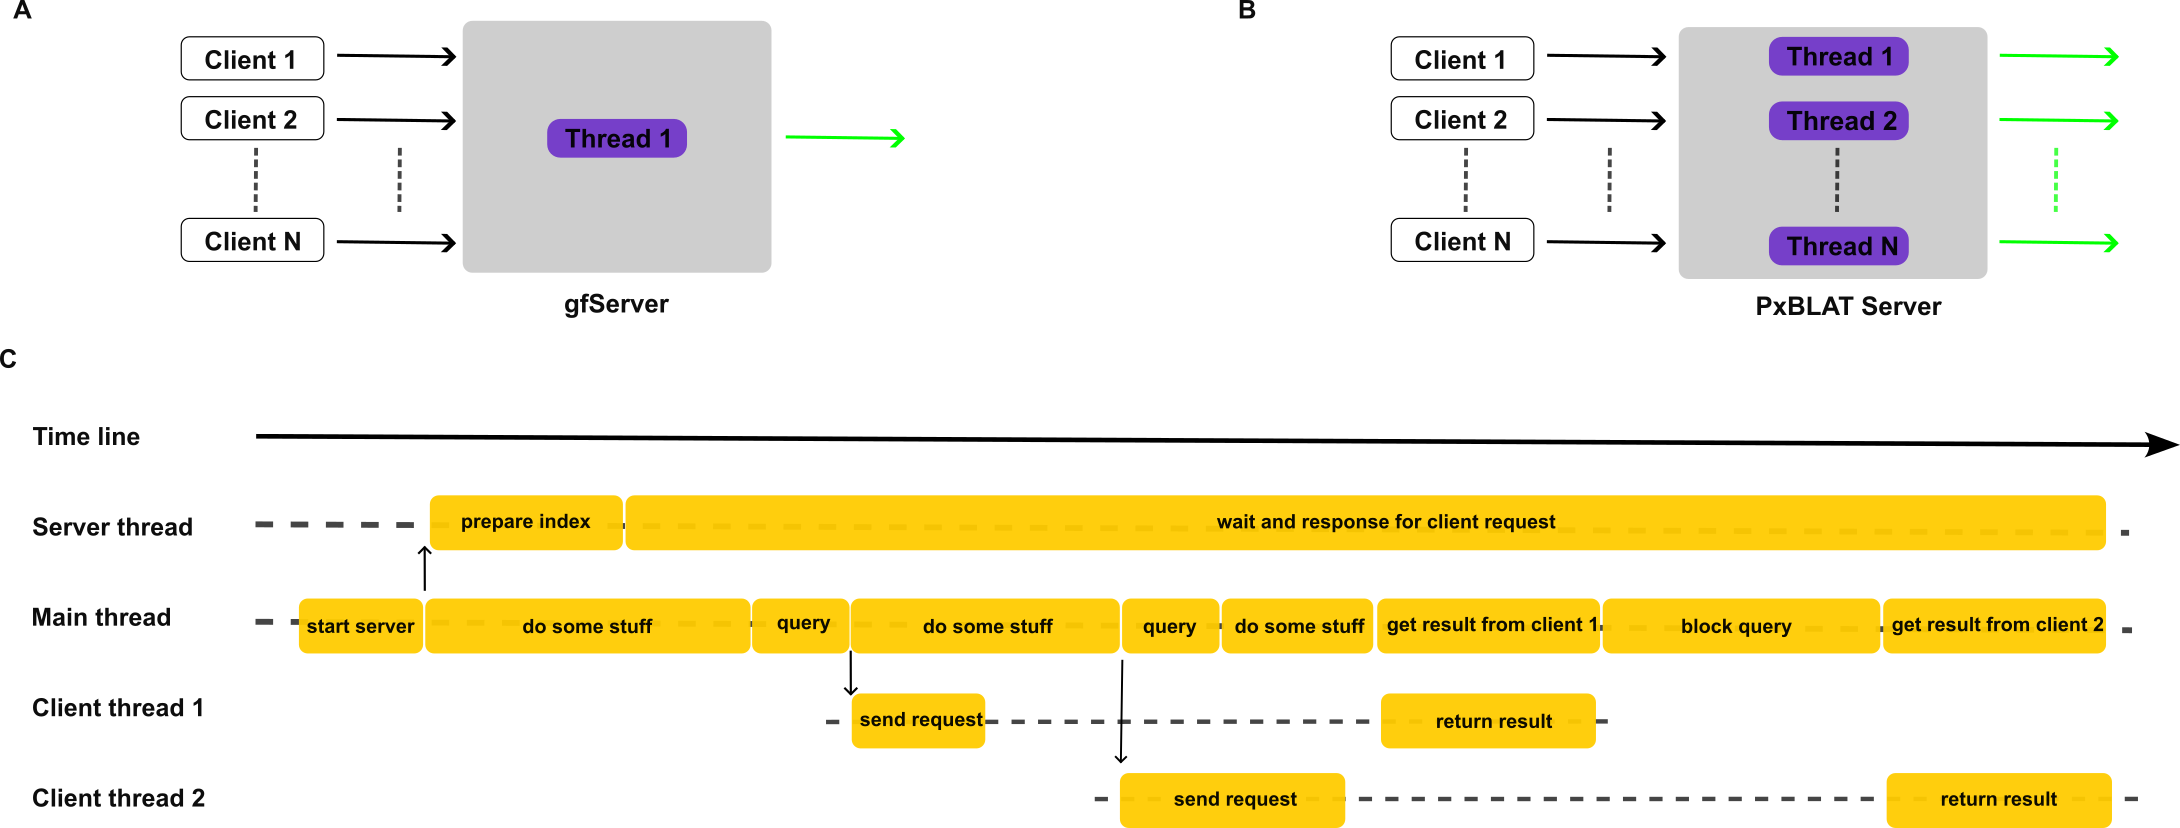
\includegraphics[width=0.75\linewidth]{figures/pxblat.png}
	\caption{\textbf{These are cells.}\\
		(\textbf{A}) This is a regular figure with a legend as a caption underneath. Inset: 3X zoom. Scale bar, \SI{10}{\micro\meter}.}
	\label{fig:pxblat}
\end{figure*}


\section*{Results}\label{sec:results}

\begin{listing}
	\inputminted[linenos]{python}{codes/example1.py}
	\caption{Python example}
	\label{listing:1}
\end{listing}


To validate \gls{pxblat}'s utility and effectiveness, we undertook a comprehensive evaluation process, assessing the library's performance, usability, and robustness.
A series of tests and comparative analysis were carried out to demonstrate the efficiency gains and ergonomic improvements offered by \gls{pxblat} over \gls{blat} usage.
We evaluated \gls{pxblat}'s efficiency by comparing the execution times of identical alignment tasks performed directly using \gls{blat}  and via \gls{pxblat}.
Our tests involved datasets of varying sizes to cover a range of typical usage scenarios.
The results indicated a significant efficiency gain when using \gls{pxblat} (Figure~\hyperref[fig:pxblat]{1D}).
In all cases, the execution time was reduced when using \gls{pxblat} compared to \gls{blat}.
The reduction in execution time ranged from \SI{1}{\percent} to \SI{1}{\percent}, clearly demonstrating the benefits of \gls{pxblat} 's direct interfacing approach.
In summary, \gls{pxblat}  offers tangible benefits in terms of reduced execution time and improved user experience, proving its value as an enhancement to BLAT's functionality.

Through our evaluation, we have demonstrated that \gls{pxblat} not only accelerates the execution of BLAT operations but also presents a user-friendly,
pythonic interface that seamlessly integrates with existing Python-based bioinformatics workflows.
While the current version of \gls{pxblat}  has demonstrated significant advantages in terms of efficiency and ergonomics, we believe that there is potential for further development and enhancement.
\gls{pxblat} represents a significant contribution in this regard, offering a blend of performance and usability that stands to benefit a wide range of users.

% Even though python cannot use multiple threads truly due to \acrfull{gil}
For gaining the power of concurrent in python, we commonly launch processes due to \gls{gil}.
The overhead of launching process is not trivial as forking a thread, but multiple threads model still empower IO operations
Compared to \gls{blat}, \gls{pxblat} benefit the characteristics to speed up multiple clients request spontaneously (Figure~\hyperref[fig:pxblat]{1A} and ~\hyperref[fig:pxblat]{1B}) since we reimplement multithreaded server in Cpp.
\gls{gil} does not exist in Cpp.



\section*{Acknowledgements}\label{sec:acknowledgements}


\section*{Conflict of interest}\label{sec:conflict-of-interest}


\section*{Funding}\label{sec:funding}


\section*{Data availability}\label{sec:data-availability}

The \gls{pxblat}, along with the source code, example scripts, and comprehensive documentation, are publicly available in our GitHub repository at \url{https://github.com/cauliyang/pxblat}.
We have also provided extensive test data, allowing users to validate the functionality and performance of \gls{pxblat} in their own environments.
We welcome community contributions to the \gls{pxblat} project.
We believe that the open availability of our data and code will foster collaboration and iterative improvement, in line with our vision of creating accessible, efficient tools for bioinformatics.

\section*{Reference}\label{sec:reference}
\bibliographystyle{bxv_abbrvnat}
\bibliography{refs.bib}

